\epigraph{The function of good software is to make the complex appear to be simple.}{--- \textup{Grady Booch}}

In this chapter we introduce a novel solution for automated refactoring candidate detection that combines self-supervised learning with pre-trained language models. Our approach moves beyond conventional metric-based methods to capture deeper code semantics, demonstrating substantial improvements in accuracy and practical applicability.


\section{Introduction}
Refactoring is a process and a set of techniques to improve source code's structure and quality without impacting the behavior and functionality of the software, thus making the software more maintainable~\cite{Opdyke1992Refactoring, Fowler1999Refactoring}. 
It is a widely used technique among software developers as it improves code readability, testability, flexibility, and adaptability to introduce changes to meet new requirements~\cite{Mens2004Survey}.

One of the critical questions that a developer answers during software development is whether a source code entity (\eg{} a method or a class) requires refactoring and if yes, what is the most appropriate refactoring in the context. 
Practitioners decide \textit{what} to refactor according to their intuition and experience. 
They can also use automated tools to calculate code quality metrics and code smells~\cite{Sharma2018}. 
However, metrics and smells focus on the \textit{problem} aspect and provide little help to decide whether and what refactoring technique must be applied to remove the smell or improve the metrics.


To overcome this challenge, many studies propose techniques to predict refactoring candidates by analyzing source code properties~\cite{Aniche2020Effectiveness, Karakati2023Software, Kurbatova2020Recommendation}.
However, existing efforts in
this direction
% the field of predicting refactoring candidates
suffers from several deficiencies. 
Currently, the state-of-the-art research in detecting refactoring candidates, 
such as Aniche \etal{}~\cite{Aniche2020Effectiveness}, 
follows a metric-based approach, \ie{} it collects code quality and process metrics, and trains a machine learning model using the collected metrics as features.
Similarly, Xu \etal{}~\cite{Xu2017}, use variable accesses in addition to code quality metrics.
These approaches fail to capture the hidden contextual and syntactical characteristics of code that might contribute to better refactoring candidate identification. 
To overcome the issue,
researchers have used code embeddings~\cite{Kurbatova2020Recommendation, Karakati2023Software} extracted from Code2Vec~\cite{Alon2019Code2vec}. 
However, existing studies in this domain do not capture rich contextual and syntactical characteristics of code~\cite{Karmakae2021Modelcoderep};
such information could significantly improve the performance of the identified refactoring candidates.
Secondly, existing studies lack an appropriate mechanism to define and identify negative samples for their dataset in this context.
A code snippet is considered a negative sample if it is not a candidate for the specific refactoring.
Typically, studies use tools such as RefactoringMiner~\cite{Tsantalis:ICSE:2018:RefactoringMiner, Tsantalis:TSE:2020:RefactoringMiner2.0} to identify positive code samples. 
% \todo{Reformatted the sentence and added ref} 
However, to identify negative samples, researchers define unsound rule-based heuristics
resulting in a low-quality noisy dataset~\cite{trautsch2023really}.
Finally, most of the previous research in this field fails to consider the real-world ratio of positive and negative samples while evaluating the predictive models. 
Ignoring this guideline
results in a model that works well in an experimental study but performs poorly when deployed in a real-world context~\cite{Sharma2021, DiNucci2018}.

% We attempt to address the deficiencies mentioned above in this paper.
In this thesis, we address the aforementioned deficiencies.
We present an automated Deep Learning (\dl{})-based technique to identify candidates for \exm{} refactoring. 
 %It specifically focuses on identifying the method level code refactoring \emph{extract method}. 
The \exm{} refactoring isolates a code block from a larger method and generates a new method based on the extracted code snippet~\cite{Fowler1999Refactoring}. 
We kept our focus on \exm{} because it is one of the most commonly used refactoring~\cite{Murphy-Hill2012}. 
We create our dataset from open-source Java repositories and 
prepare an effective code representation capturing syntactic and semantic properties of methods by combining \GCB{}~\cite{Guo2020GraphCodeBERT} and Autoencoder~\cite{Liou2014Autoencoder}.
The representation is then used to identify \exm{} refactoring candidates.

\textit{Contributions of the study:}
% \begin{itemize}
%     \item
    We propose a novel mechanism to properly identify positive and negative samples for \exm{} refactoring.
    The mechanism helps us create a dataset containing $55,430$ positive and negative samples that serves as a benchmark for automated refactoring candidate identification approaches properly.
  To study the effectiveness of the method representation generated using \GCB{} in a binary classification task, we propose an Autoencoder-based approach to identify latent features.


\textbf{Replication package:} We made our code~\cite{ExtractMethodIdentificationRepo} publicly available with our training data~\cite{indranil_palit_2023_8122619} for easier replication and use.


 


 




\section{Approach}
This section describes the experimental approach followed to investigate the potential of Large Language Models (\llm{}s) in determining the suitability of a method for \textit{extract method} refactoring.

\begin{figure*}
\centering
%\noindent
\centerline{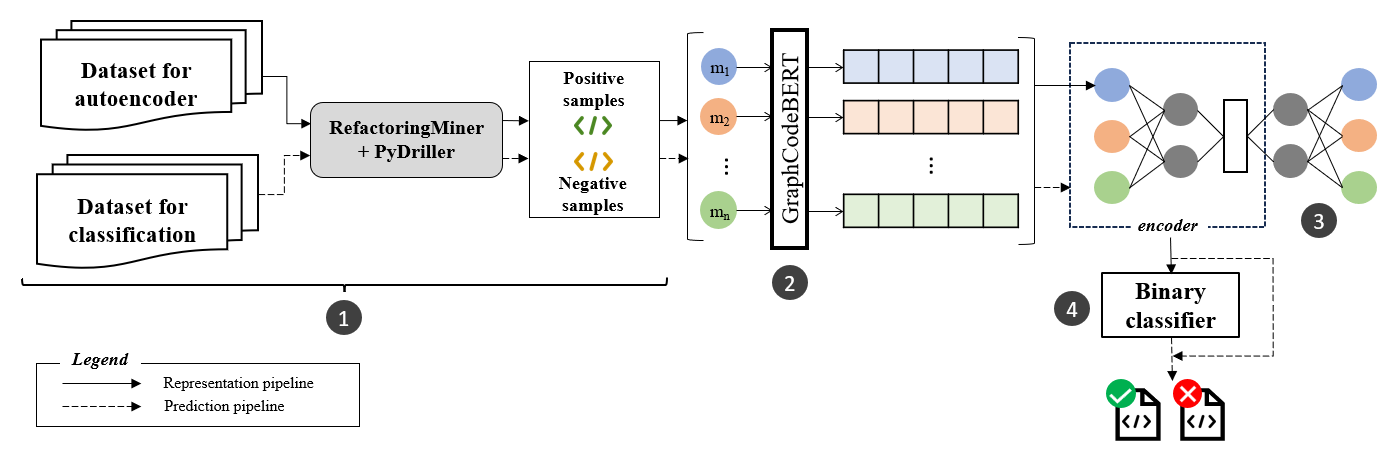
\includegraphics[width=\textwidth]{chapters/identification/Images/ArchDiagram.png}}
\caption{Overview of the proposed approach}
\label{fig:methodology}
% \vspace{-5pt}
\end{figure*}
\subsection{Overview}
The study aims to develop a \dl{}-based \exm{} refactoring candidate identification technique that addresses the deficiencies in the existing studies.
Figure~\ref{fig:methodology} presents an overview of our approach.
We first pick a set of repositories to prepare our dataset.
We use existing tools RefactoringMiner~\cite{Tsantalis:ICSE:2018:RefactoringMiner} and PyDriller~\cite{Spadini2018}, to segregate methods into positive and negative samples.
Our approach utilizes \GCB{} to generate embeddings for each sample.
We employ a \dl{} model based on Autoencoder~\cite{Liou2014Autoencoder} that is used for feature extraction and dimensionality reduction. 
We utilize the encoder component of the trained Autoencoder to generate a lower-dimensional latent space representation from the initially high-dimensional embedding input. 
The representation obtained from the bottleneck layer of Autoencoder is then used as a feature vector to train a \rf{} (\RF{}) classifier on the \exm{} identification task.
We formulate the following research questions.
% to evaluate the effectiveness of the proposed approach. 


\begin{itemize}
    \item [\textbf{RQ1}] 
    \textit{How does our proposed approach perform compared to the state-of-the-art?}
    % \smallskip
\end{itemize}    

    By answering this research question, we intend to evaluate and validate the performance of the proposed approach as compared to the
    % \todo{added -}
    state of the art. 


    \begin{itemize}
    \item 
    [\textbf{RQ2}] \textit{How effectively does the autoencoder extracts features for the classification task?}
\end{itemize}    
    In this research question,
    we aim to evaluate the effectiveness of the employed autoencoder-based model by extracting the learned features and using them for the classification task.


\subsection{Dataset preparation}
\label{dataset_prep}

We utilized a subset of repositories ($5$\%) from the $11,149$ open-source Java repositories used by Aniche~\etal{}~\cite{Aniche2020Effectiveness}, as working with the entire set required extensive computing infrastructure. This initial selection yielded $558$ repositories, from which we excluded repositories that were no longer available on GitHub or lacked any instances of \exm{} refactoring throughout their history. After filtering, we obtained $410$ repositories with at least one \exm{} refactoring performed. 
To leverage a trained autoencoder and using the trained encoder of the autoencoder for the classification task without data leakage, we divided this dataset into two parts: one for autoencoder pipeline with $208$ repositories and the remaining $202$ for the classification pipeline.



% \subsubsection{Dataset preparation}
As shown in step~\circled{1} of Figure~\ref{fig:methodology},
we use RefactoringMiner, a state-of-the-art refactoring detection tool~\cite{Tsantalis:ICSE:2018:RefactoringMiner, Tsantalis:TSE:2020:RefactoringMiner2.0} to prepare our dataset.
This tool reports performed refactorings, if any, 
in each commit within a Java repository's history. 
It provides essential metadata such as the code component involved (\eg{} method start line and end line in the case of \exm{} refactoring) and the associated commit hash. Leveraging this information, we utilize PyDriller~\cite{Spadini2018} to iterate through the identified commits and extract source code of the involved methods.


We identify positive samples where \exm{} refactoring has been applied following the mechanism described above.
Identifying negative samples for \exm{} refactoring is a challenging task. Merely excluding methods not reported by RefactoringMiner is insufficient since the absence of refactoring does not guarantee a method is not a refactoring candidate. Previous work have proposed heuristics-based approaches to address this challenge. For instance, Aniche~\etal{}~\cite{Aniche2020Effectiveness} used a criterion based on the method's modification history, while Yamanaka~\etal{}~\cite{Yamanaka2021RecommendingEM} selected code portions that differ from actual extractions. 
However, these heuristics may introduce noise and create sub-optimal datasets by misclassifying potential \exm{} candidates.

We propose a new mechanism to identify negative samples for the study. A method is considered a negative sample in commit $C_{n}$ if it underwent \exm{} refactoring in its parent commit $C_{n-1}$.  
The rationale behind this idea is that it is highly unlikely that a method that underwent \exm{} refactoring will again go through the same refactoring. This reduces the risk of false negative detection and ensures a high quality dataset. 
The aforementioned approach of identifying positive and negative samples, resulted in $27\small,634$ and $27\small,796$ samples for training and evaluating the Autoencoder, and  binary classifier respectively. Table~\ref{tab:ident_dataset_stats} describes the dataset statistics used to train, test and validate our approach.

\begin{table}[ht!]
    \centering
    \caption{Dataset statistics} \label{tab:ident_dataset_stats}
        \begin{tabular}{cccc|cccc}
            \toprule
            \multirow{2}{*}{Dataset} & \multicolumn{3}{c}{Positive samples} & \multicolumn{3}{c}{Negative samples} \\
            \cmidrule(lr){2-7}
& \makecell[c]{Avg.\\ LOC} &  \makecell[c]{Avg. \\ token\\ length} &  \makecell[c]{Median \\ LOC} &  \makecell[c]{Avg.\\ LOC} &  \makecell[c]{Avg.\\ token\\ length} &  \makecell[c]{Median \\ LOC} &\\
            \cmidrule(lr){1-7}
\makecell[l]{Train split}& $36.46$ & $343.26$ & $14$ & $26$ & $25.23$ & $263.24$\\ \addlinespace
\makecell[l]{Test split} & $36.22$ & $341.57$ & $14$ & $26$ & $24.46$ & $261.55$ \\ \addlinespace
\makecell[l]{Val split} & $35.57$ & $338.88$ & $13$ & $26$ & $25.50$ & $268.27$ \\ \addlinespace
% \makecell[l]{$\mathcal{D}$} & 411.68 & 447.69 & 185.94 & 241.88 \\ 
            \bottomrule
        \end{tabular}    
\end{table}
\vspace*{\fill}


\subsection{Data representation}

In step~\circled{2}, we use \GCB{} to capture both syntactic and semantic information of code, providing a comprehensive representation of code snippets by using graph-guided masked attention function to incorporate the code structure. 
The initial step in processing the input code through the \GCB{} model involves tokenization and encoding. To accomplish this, we utilize the pre-trained \GCB{} tokenizer.
% The \GCB{} model anticipates an input sequence of tokens, which must begin with a special \texttt{[CLS]} token and conclude with another special token, \texttt{[SEP]}. 
To ensure the token sequence adheres to the model's maximum length of $512$, we truncate it if it surpasses this limit. 
Subsequently, we perform batch encoding on the token sequence, generating \texttt{input\_ids} which represent the tokens numerically for the model. 

To extract the embeddings, we pass this encoded input to \GCB{}. 
During the forward propagation of the input, each of the $12$ hidden layers of the model generates individual token embeddings based on the surrounding context. To get the condensed representation of the sequence of tokens, we use mean pooling. We conducted a pilot study and we found that this approach performs better than taking the embedding of the \texttt{[SEP]} token alone.
This results in a single embedding vector of size $768$ for each of the input sample. We consider this as our feature vector for the classification task.

% \vspace{-1mm}

\subsection{Model training and classification}


\subsubsection{Autoencoder}

We use the generated embeddings from \GCB{} as the input for training the autoencoder model (step~\circled{3}). 
The architecture of the autoencoder that we trained consists of an encoder with three fully connected linear layers and ReLU activation to learn the hidden representation that reduces the input dimension to a bottleneck layer of size $128$. The decoder reverses this process to reconstruct the original input of size $768$. The autoencoder model is trained on $70\%$. The rest $30\%$ is used to validate the model. We calculate the reconstruction loss using \textit{Mean Squared Error} (MSE) loss.


\subsubsection{Binary classifier}
After training the autoencoder, in step~\circled{4}, we take the \textit{encoder} part of the trained model and use it as our feature extractor for the binary classification dataset.
We train two classifiers---a traditional machine learning model \rf{} and a \dl{}-based feed forward neural network, and compare their performance. 
We chose to use \rf{}
due to its ensemble learning method for classification and its ability to learn the non-linear relationship between the features,
\rf{} has shown to perform very well in different software engineering tasks~\cite{DiNucci2018, Immaculate2019} including refactoring identification~\cite{Aniche2020Effectiveness,VanDerLeij2021Data}. 

To train our models, 
we first split the $27,796$ samples into train, validation, and test sets in $70:10:20$ ratio 
using stratified sampling. 
We use \textit{GridSearchCV}
to select the optimal hyper-parameters for \rf{}.
The optimal set of hyper-parameter values along with their search space is reported in Table~\ref{tab:rfparams}
The neural network classifier consists of two fully connected layers with ReLU activation and a final sigmoid activation layer.

\begin{table*}[ht]
\captionsetup{skip=10pt}
\centering
\caption{Optimal hyper-parameter values for random forest}
\label{tab:rfparams}
\rowcolors{2}{gray!25}{white}
\begin{tabular}{p{5cm}%
>{\raggedleft\arraybackslash}p{4cm}%
>{\raggedleft\arraybackslash}p{4cm}%
}
\textbf{Parameter} & \textbf{Search space} & \textbf{Best value} \\ \midrule
Number of trees & ${[}100, 200, 300, 1000{]}$ & $1000$ \\
Minimum samples split    & ${[}8, 10, 12{]}$           & $10$   \\
Minimum leaf node samples              & ${[}3, 4, 5{]}$             & $3$    \\
Maximum features              & ${[}2, 3{]}$                & $2$    \\
Maximum tree depth                    & ${[}80, 90, 100, 110{]}$    & $80$  \\\bottomrule
% \vspace{-5pt}
\end{tabular}
\end{table*}

\subsubsection{Evaluation}

To evaluate our models, we calculate the \textit{accuracy, precision, recall,} and \textit{F1 score}.


Initially, the test split of our classification dataset, 
contains positive and negative samples in equal proportion. 
However, it has been argued~\cite{Sharma2021, DiNucci2018} that a test set not representative of the real-world may show good performance while experimentation 
but do poorly when deployed in a real-world scenario. 
To address this issue, 
we identify the ratio of positive and negative samples in the following manner. 
First, we sample $20$ repositories from our dataset randomly. 
For each of the selected repositories, we identify the commits in which \exm{} refactoring has been applied using RefactoringMiner along with the count of such methods ($posCount$). 
Using PyDriller, we identify the count of total methods present in the source code for that commit ($totalCount$). 
Then we compute the ratio $\frac{posCount}{totalCount}$ and take the mean across all identified commits to find a real-world ratio of \exm{} refactoring candidates. 
We modify the test set  to represent the computed ratio ($85:15$) and then perform the evaluation. 


\section{Experimental Results}
\noindent
\textbf{RQ1}: \textit{How does our proposed approach perform compared to
the state-of-the-art?}




In this research question, we compare our two approaches \texttt{M1} (\ie{} neural network-based classification) and \texttt{M2} (\ie{} \rf{}-based classification), where both the models utilize GraphCodeBERT and Autoencoder to generate latent representation.
We compare the results from our models
against state-of-the-art approach from Aniche \etal{} \cite{Aniche2020Effectiveness}.
Though the baseline study compare many machine learning techniques,
we chose to compare our models with only their \rf{} model because it reported the best results in that study.
All of the models we tested using the same test split.
% as described in Section~\ref{dataset_prep}. 

\begin{table}[ht]
\centering
\caption{Experimental results for RQ1}
\label{tab:exresults}
\rowcolors{2}{gray!25}{white}
\begin{tabular}{p{4cm}|%
>{\raggedleft\arraybackslash}p{2cm}%
>{\raggedleft\arraybackslash}p{2cm}%
>{\raggedleft\arraybackslash}p{2cm}%
>{\raggedleft\arraybackslash}p{2cm}%
}
\textbf{Models} & \textbf{Accuracy} & \textbf{Precision} & \textbf{Recall} & \textbf{F1-score} \\ \midrule
M1 (GraphCodeBERT + Autoencoder + Neural Network) & $0.57$ & $0.71$ & $0.57$ & $0.63$ \\
M2 (GraphCodeBERT + Autoencoder + Random forest) & $\mathbf{0.87}$ & $\mathbf{0.90}$ & $\mathbf{0.87}$ & $\mathbf{0.88}$  \\
Baseline (with random forest) & $0.84$ & $0.44$ & $\mathbf{0.87}$ & $0.58$ \\\bottomrule
\end{tabular}
\end{table}


Table~\ref{tab:exresults} presents results of our experiments.
From the results it is evident that our \texttt{M2} model outperforms the baseline as well as the \texttt{M1} model. 
We observe that both \texttt{M1} and \texttt{M2} outperform the baseline. Specifically, we see that \texttt{M2} outperform the \rf{} used by Aniche~\etal{} by nearly 50\% in terms of precision.
At the same time, our model \texttt{M2} exhibits a good recall rate of $0.87$.
Consequently, we see that our model 
performs significantly better than the considered baseline model by approximately $30\%$ in terms of F1 score.


\begin{boxH}
\textbf{RQ1 Summary:} 
Our results show that our \rf{}-based model outperforms the baseline model significantly (by $30\%$, in terms of F1 score).
The results indicate that our  code representation is successfully capturing syntactic and semantic characteristics of code necessary to identify \exm{} refactoring candidates.
\end{boxH}

\noindent
\textbf{RQ2}: \textit{How effectively does the autoencoder extracts features for the classification task?}
% \vspace{0.3mm}

We train an autoencoder model and use the trained encoder part of it as a feature extractor.
We do so to reduce the vectors' dimensionality and extract relevant features from the embeddings generated from \GCB{}. 

\begin{figure}[htbp]

\begin{minipage}[t]{0.49\linewidth}
    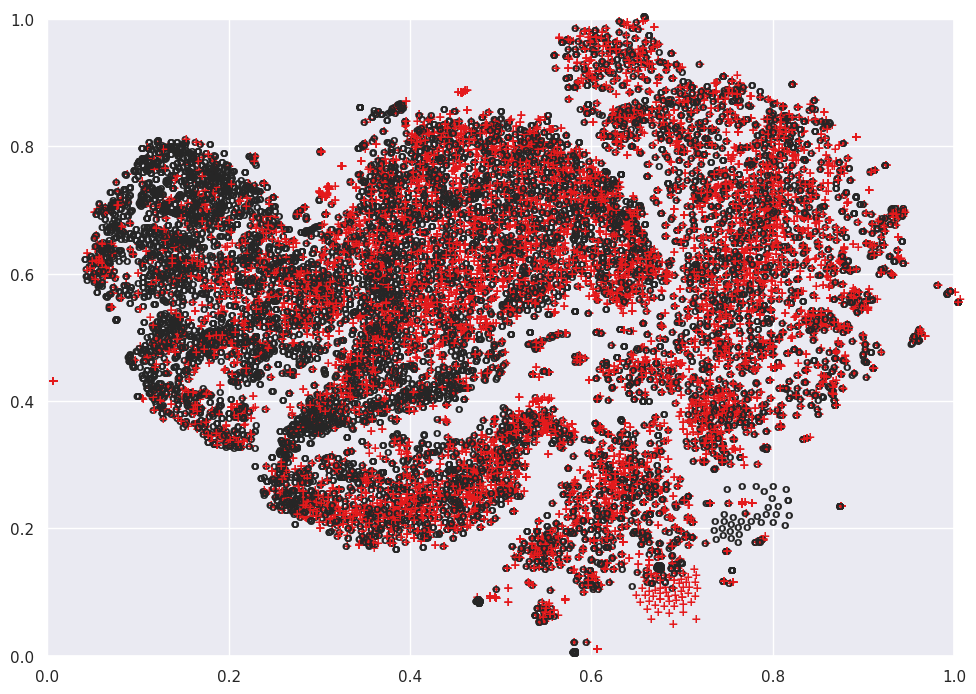
\includegraphics[width=\linewidth]{chapters/identification/Images/tsne_gc.png}
    \caption{Class separation with embeddings (from \GCB{})}
    \label{embonly}
\end{minipage} 
    \hfill%
\begin{minipage}[t]{0.49\linewidth}
    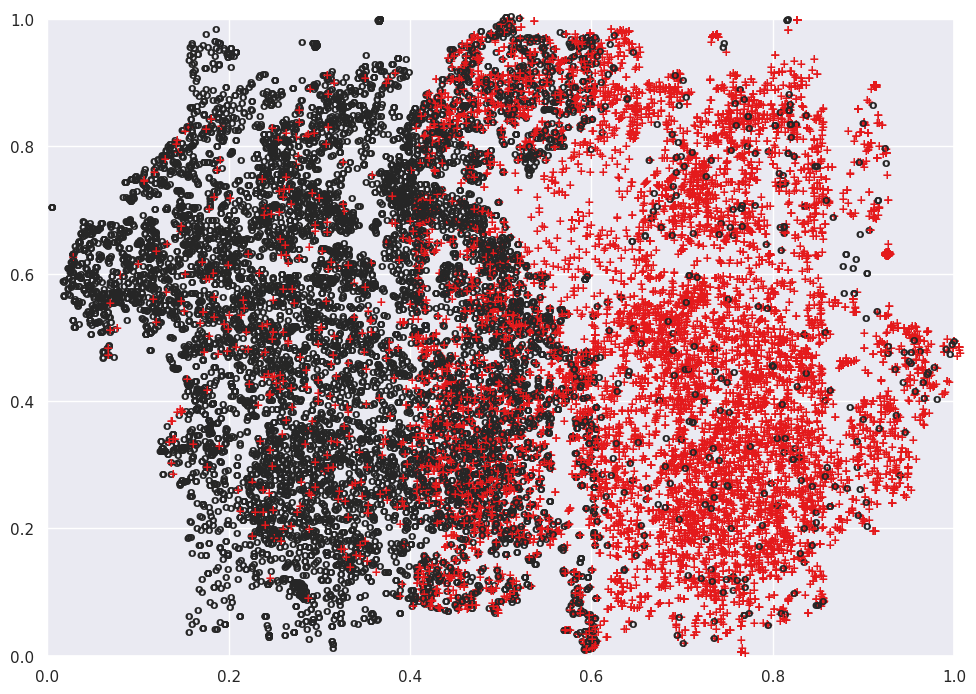
\includegraphics[width=\linewidth]{chapters/identification/Images/tsne_ae_1.png}
    \caption{Class separation with encoded embeddings (from Autoencoder)}
    \label{encodedemb}
\end{minipage}%

\end{figure}


% As we can see from the curve, the model performs well at reconstructing the input embeddings with minimum loss. 
To measure the performance and usefulness of the trained autoencoder model as a feature extractor, we first analyze the \texttt{t-SNE}~\cite{van2008visualizing} plots of the embeddings generated by \GCB{} and those generated by the combination of \GCB{} and Autoencoder. We do so to study the class separability. The distinguishability of classes in the \texttt{t-SNE} space is assessed through a clear separation and quantified by calculating the Euclidean distance between the centroids of each class. Figure~\ref{encodedemb} shows a reasonably clear bifurcation between the classes with an euclidean distance of $0.367$ as compared to $0.122$ for Figure~\ref{embonly}. We can infer that a classification model trained on the encoded embedding will perform better than the one trained on embeddings alone. This observation can be attributed to the autoencoder being able to learn hidden features unique to each type of sample which helps it to segregate them.

To further investigate the effectiveness of these representations, we perform an ablation study where we train classifier with and without the autoencoder representation of the embeddings. 
% In the first case, we train and test the model directly with the embeddings generated by \GCB{}. 
% In another case, after generating the initial embeddings for the training set from \GCB{}, we encode them using the trained encoder part of the autoencoder model. 
We report the performance results in Table~\ref{tab:emcomp}.
% The evaluation metrics are computed and reported in Figure~\ref{fig:aechart} for a comparative analysis. 
The \rf{} classification model, when trained with the encoded representation of the embedding provided by Autoencoder, 
outperforms the one trained with only the \GCB{} embedding vector as features. 
% While we observe a slight increase of \textbf{$7\%$} in terms of Precision metric value, there's a significant increase of about \textbf{$28\%$} on average for the other 3 metrics. 
These findings support our claim that the
autoencoder extracts features and reduces dimensionality effectively
in the context of refactoring candidate identification.

\begin{boxH}
\textbf{RQ2 Summary:} Autoencoder-encoded code representations from \GCB{} significantly improve classification performance compared to \GCB{} representations alone.
\end{boxH}


\begin{table}[h!]
\centering
\caption{Encoded embedding performance}
\label{tab:emcomp}
\rowcolors{2}{gray!25}{white}
\begin{tabular}{p{4cm}|%
>{\raggedleft\arraybackslash}p{2cm}%
>{\raggedleft\arraybackslash}p{2cm}%
>{\raggedleft\arraybackslash}p{2cm}%
>{\raggedleft\arraybackslash}p{2cm}%
}
\textbf{Models} & \textbf{Accuracy} & \textbf{Precision} & \textbf{Recall} & \textbf{F1-score} \\ \midrule
\begin{tabular}[c]{@{}l@{}}Embeddings\end{tabular} & $0.57$ & $0.71$ & $0.57$ & $0.63$ \\
\begin{tabular}[c]{@{}l@{}}Encoded embeddings\end{tabular}  & $\mathbf{0.87}$ & $\mathbf{0.90}$ & $\mathbf{0.87}$ & $\mathbf{0.88}$ 
% Baseline (with random forest) & 0.84 & 0.44 & \textbf{0.87} & 0.58
\\\bottomrule
\end{tabular}
\end{table}

% \section{Related Work}
% % \todo{are there studies that identify refactoring candidate without using machine learning? If yes, we need a subsection for them.}

\subsection{Refactoring candidate identification using traditional techniques}

Software developers can manually decide \textit{what} to refactor according to their intuition and past experiences~\cite{Al2015Identifying}.
Often, they use automated tools to calculate code quality metrics and code smells to identify refactoring candidates~\cite{Mens2004Survey, Al2015Identifying}. 
Another method to identify refactoring candidates is to define a set of preconditions or compliance rules. If a code did not follow these rules, it was considered a candidate for refactoring. Studies by Bois \etal{}~\cite{Du2004Refactoring} and Kataoka \etal{}~\cite{Kataoka2001Automated} used such compliance rules.

Another technique considers creating clustering algorithms to identify if code needs refactoring. 
Czibula \etal{}~\cite{Czibula2008Hierarchical} and Serban \etal{}~\cite{Serban2007Restructuring}, 
created clusters based on the distance between methods and attributes within and outside of classes to identify numerous refactoring candidates.
Similarly, Bavota \etal{}~\cite{Bavota2011Identifying} suggest a graph-based approach that uses weighted graphs instead of abstract syntax trees to identify methods that can be extracted. 
Finally, Tsantalis \etal{}~\cite{Tsantalis2009Identification} used code slices to identify \exm{} candidates.

\subsection{Detecting refactoring with Machine Learning techniques}

Many studies have explored ways to identify refactoring candidates automatically using machine learning.
Typically, such studies use
source code metrics or commit messages to train a model. For example, Aniche \etal{}~\cite{Aniche2020Effectiveness} predict $20$ kinds of refactorings at the method, class, or variable level. 
They use a large number of code, process, and ownership metrics to train six supervised machine learning algorithms. 
The study reports that \rf{} model performs the best among the compared models.
Gerling~\cite{Gerling2020Machine} conducted an empirical study as an extension of Aniche \etal{}'s study. 
They focused on improving the data collection process in Aniche \etal{}'s study to create a high quality large-scale refactoring dataset. 


Similarly, Van Der Leij \etal{}~\cite{VanDerLeij2021Data} analyze five machine learning models to predict \exm{} refactoring and compare the results with industry experts.
They collect $61$ code metrics and analyze \rf{}, \dt{}, \logr{}, Linear \SVM{}, and Gaussian \nb{} algorithms. 
They found \rf{} as the best performing model. 
Kumar \etal{}~\cite{Kumar2019Method} perform a study to predict method-level refactoring and analyze $10$ machine learning classifiers. 


Sagar \etal{}~\cite{Sagar2021Comparing} considers the problem of refactoring candidate prediction as a multi-class classification problem. 
Their study uses source code quality metrics and commit messages as features to predict six method-level refactorings. 
They compare two machine learning models: a text-based model that analyses keywords from commit messages and a source code-based model that analyses $64$ code quality metrics. 
Kurbatova \etal{}~\cite{Kurbatova2020Recommendation} use code embeddings generated from Code2Vec~\cite{Alon2019Code2vec} to train their machine learning model to predict the \mm{} refactoring. 



\section{Threats to Validity}
\noindent
\textbf{Construct validity:} 
Construct validity measures the degree to which tools and metrics actually measure the properties that they are supposed to measure. 
It concerns the appropriateness of observations and inferences based on measurements taken during the study.
The quality of positive and negative samples extracted from RefactoringMiner and PyDriller poses a threat to validity.
Though RefactoringMiner and PyDriller are state-of-the-art tools that are widely used and considered accurate,
to mitigate the threat,
we randomly picked up a subset of the identified negative samples and manually evaluated the quality of the samples.


Our approach uses a significantly smaller dataset (approximately $5\%$) compared to the dataset used in the state-of-the-art approach.
Though the chosen repositories are representative,
it can be considered a threat to validity.
We chose the smaller dataset
because of the computing resources required for the full-size dataset. 
Additionally, in this study, we aimed to explore the feasibility and effectiveness of the proposed approach.
In the future, we aim to repeat the experiment with a larger dataset.

\noindent
\textbf{External validity:}
External validity concerns the generalizability and repeatability of the produced results.
One of the threats to validity in this thesis is that the approach proposed is exclusive to \exm{} refactoring. 
Using our approach for another kind of refactoring is challenging and requires extensive reworking of the approach used. 
For example, \emph{move method} refactoring moves a method to an appropriate class~\cite{Fowler1999Refactoring}. 
We cannot apply the same approach that we adopted to create \exm{} dataset for \emph{move method} refactoring
because we will not have the code to collect in the refactored commit since the method would have moved to another class. 
A similar challenge is expected when considering other refactoring types, such as \emph{pull up method} and \emph{push down method}.
In the future, we would like to address this challenge and propose an effective and generic dataset-creation approach for different refactoring types.
